\appchapter{建立模型}
在本节中,我们将将详细介绍旋转运动过程中的摩擦模型和动力学模型。
我们用角度 $\theta$ 表示物体相对于夹持器的位置,如图 2 所示。
旋转的目的是将被抓取的物体从初始位置 $\theta_0$ 旋转到期望的位置 $\theta_d$ 。
我们通过改变指尖产生的摩擦力矩 ${\tau _f}$控制物体的旋转运动。
我们假设夹持器有一个自由度,有两个柔软的半球形指尖,
物体围绕连接指尖的固定旋转轴旋转。

\begin{figure}[!ht]
  \centering
  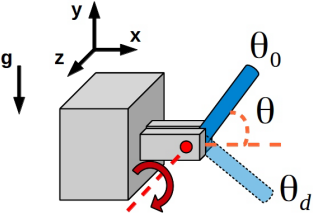
\includegraphics[scale=0.9]{appendices/pic/3-1}
  \caption*{
    \mtb{图2}旋转任务的建模。重力矢量用 $g$ 表示,
    $\theta$ 是物体与夹持器之间的相对位置,
    $\theta$ 、 $\theta_d$ 分别表示初始和期望的角度位置。}
  \vspace{-0.3cm}
\end{figure}

我们在前人对柔性手指力学建模研究的基础上,建立了旋转过程中的扭转摩擦模型。
这些模型建立了指尖的扭转摩擦力与其所施加的握力之间的关系,
我们将在控制方案设计中使用。
假设夹持器处于固定位置,则物体的运动仅由其重力矩和摩擦力矩决定。

\appsection{软指接触模型}
机器人手的指尖接触模型根据其摩擦特性一般可分为三类:无摩擦的硬指接
触、有摩擦的硬指接触和软指接触$^{[20, 21]}$。软指接触模型假定手指可以施加与
接触面相切的摩擦力以及垂直于接触面方向的摩擦力矩。此外用一个柔软的手指
抓住物体,直到物体发生滑动的过程中,可以施加在物体上的最大的力和力矩之间
存在一种非线性关系$^{[11, 12, 17]}$。
这个最大的力和力矩的边界称为极限面,可以用椭球体来近似$^{[4]}$

\stepcounter{appequ}
\vspace{-15pt}
\begin{equation}
  {f^T}Af = 1
\end{equation}

\noindent 其中$f = \left[ {{f_x},{f_y},{\tau _z}} \right]$ 表示接触处的摩擦力旋,
$\left( {{f_x},{f_y}} \right)$ 为切向摩擦力分量,
${\tau _z}$ 为法向摩擦力矩。
假设各向同性摩擦,矩阵$A \in {R^{3 \times 3}}$变为对角矩阵 ,
其元素为最大摩擦力和力矩

\stepcounter{appequ}
\vspace{-15pt}
\begin{equation}
  A = diag\left( {f_{t,\max }^{ - 2},f_{t,\max }^{ - 2},\tau _{z,\max }^{ - 2}} \right)
\end{equation}

\noindent 其中, 最大切向力 $f_{t,max}$可 由 库 仑 摩 擦 表 示

\stepcounter{appequ}
\vspace{-15pt}
\begin{equation}
  {f_{t,\max }} = \mu {f_n}
\end{equation}

\noindent 式中, $\mu$ 为摩擦系数, $f_n$ 为施加在触点法向上的压力。
另一方面,被抓取物体旋转前的最大扭转摩擦${\tau _{z,\max }}$  更加复杂,
它的大小和方向取决于接触面的几何形状和压力分布。
我们假设被抓取的物体在接触点有一个局部光滑的表面,使得接触面是圆形的。
那么最大摩擦力矩遵循类库仑模型$^{[12, 22]}$

\stepcounter{appequ}
\vspace{-15pt}
\begin{equation}
  {\tau _{z,\max }} = \alpha \beta \mu {f_n}
\end{equation}

其中 $\alpha$ 是接触面半径,常数 $\beta$ 取决于局部压力分布。
例如对于赫兹压力分布,该参数可取 $\beta = 0.589$ ;
对于均匀分布,该参数可取 $\beta= 0.667$ $^{12]}$。

当施加在物体上的合外力旋包含在椭球体极限面内(即 $f_{ext}^TA{f_{ext}} < 1$)时,
物体保持静止。一旦物体开始滑动,极限面模型假设摩擦力旋仍然保持在极限面上,
该力旋产生的滑动速度垂直于椭球体。
在我们的项目中,我们假设物体被抓得离它的质心足够远,
因此重力矩比物体的重力对运动产生的影响更显著。
因此,物体的平移运动相对于其旋转运动可忽略不计,
摩擦力矩 $\tau_f$ 近似等于式(4)中的$\tau_{z,max}$

\stepcounter{appequ}
\vspace{-15pt}
\begin{equation}
  {\tau _f} = \alpha \beta \mu {f_n}
\end{equation}

值得注意的是,极限面模型忽略了潜在的与相对速度有关的滑动摩擦现象,
如 Stribeck 效应和粘性摩擦。
尽管存在这一局限性,但与以往工作$^{[4]}$所采用的方法类似,
我们在控制器设计中假设等式(5)所述的模型只考虑旋转过程中滑动摩擦力矩最主要的部分,
即假设该力矩只依赖于所施加的正压力。


为了完成我们的模型,我们还需要一个变形模型,它建立法向力$f_n$ 和接触半径a的关系。
Xydas 等人已经证明半球形指尖遵循幂律变形模型$^{[22]}$

\stepcounter{appequ}
\vspace{-15pt}
\begin{equation}
  a = cf_n^\gamma
\end{equation}

\noindent 其中 $c$ 是常数,指数 $\gamma$ 的值介于0和1/3之间,具体值取决于指尖材料。
将(6)代入(5)中,我们得到以下摩擦力矩模型

\stepcounter{appequ}
\vspace{-15pt}
\begin{equation}
  {\tau _f} = {\mu _{tors}}f_n^{1 + \gamma }
\end{equation}

式中,我们将${\mu _{tors}} = c\beta \mu $ 表示为扭转摩擦系数 。



\appsection{旋转动力学}

假设机械臂处于静止状态,物体运动过程中的旋转动力学由重力矩和摩擦力矩决定。
图 2 所示的物体绕 z 轴转动的动力学方程可由下式表示

\stepcounter{appequ}
\vspace{-15pt}
\begin{equation}
  I\ddot \theta  = {\tau _g} + {\tau _{{f_1}}} + {\tau _{{f_2}}}
\end{equation}

\noindent 式中, $I$ 是物体绕旋转轴的转动惯量, $\ddot \theta$ 是物体转动的角加速度,
$\tau_g$ 是物体的重力在转轴处产生的力矩,
${\tau _{{f_i}}}$与$i \in \left[ {1,2} \right ]$
分别表示被控物体在与两个指尖接触处产生的摩擦力矩。

我们假设抓取是对称的,使得每个手指在物体上施加的法向力相等,
并且两个指尖具有相同的变形和摩擦参数,则 ${\tau _{{f_1}}} = {\tau _{{f_2}}}$ 。
如果如图 2 所示重力沿 $y$ 轴方向,即
$\mathord{\buildrel{\lower3pt\hbox{$\scriptscriptstyle\rightharpoonup$}}
  \over g}  = g\mathord{\buildrel{\lower3pt\hbox{$\scriptscriptstyle\rightharpoonup$}}
\over y} $,代入摩擦力矩模型(7),
那么我们可以得到以下非线性旋转动力学方程

\stepcounter{appequ}
\vspace{-15pt}
\begin{equation}
  I\ddot \theta  =  - mg{l_{cm}}\cos \theta  + 2{\mu _{tors}}f_n^{1 + \gamma }
\end{equation}

\noindent 其中 $m$ 是物体的质量, $g$ 是重力, $l_cm$ 是旋转轴和物体质心之间的距离。

